\documentclass{article}\usepackage[]{graphicx}\usepackage[]{color}
%% maxwidth is the original width if it is less than linewidth
%% otherwise use linewidth (to make sure the graphics do not exceed the margin)
\makeatletter
\def\maxwidth{ %
  \ifdim\Gin@nat@width>\linewidth
    \linewidth
  \else
    \Gin@nat@width
  \fi
}
\makeatother

\definecolor{fgcolor}{rgb}{0.345, 0.345, 0.345}
\newcommand{\hlnum}[1]{\textcolor[rgb]{0.686,0.059,0.569}{#1}}%
\newcommand{\hlstr}[1]{\textcolor[rgb]{0.192,0.494,0.8}{#1}}%
\newcommand{\hlcom}[1]{\textcolor[rgb]{0.678,0.584,0.686}{\textit{#1}}}%
\newcommand{\hlopt}[1]{\textcolor[rgb]{0,0,0}{#1}}%
\newcommand{\hlstd}[1]{\textcolor[rgb]{0.345,0.345,0.345}{#1}}%
\newcommand{\hlkwa}[1]{\textcolor[rgb]{0.161,0.373,0.58}{\textbf{#1}}}%
\newcommand{\hlkwb}[1]{\textcolor[rgb]{0.69,0.353,0.396}{#1}}%
\newcommand{\hlkwc}[1]{\textcolor[rgb]{0.333,0.667,0.333}{#1}}%
\newcommand{\hlkwd}[1]{\textcolor[rgb]{0.737,0.353,0.396}{\textbf{#1}}}%
\let\hlipl\hlkwb

\usepackage{framed}
\makeatletter
\newenvironment{kframe}{%
 \def\at@end@of@kframe{}%
 \ifinner\ifhmode%
  \def\at@end@of@kframe{\end{minipage}}%
  \begin{minipage}{\columnwidth}%
 \fi\fi%
 \def\FrameCommand##1{\hskip\@totalleftmargin \hskip-\fboxsep
 \colorbox{shadecolor}{##1}\hskip-\fboxsep
     % There is no \\@totalrightmargin, so:
     \hskip-\linewidth \hskip-\@totalleftmargin \hskip\columnwidth}%
 \MakeFramed {\advance\hsize-\width
   \@totalleftmargin\z@ \linewidth\hsize
   \@setminipage}}%
 {\par\unskip\endMakeFramed%
 \at@end@of@kframe}
\makeatother

\definecolor{shadecolor}{rgb}{.97, .97, .97}
\definecolor{messagecolor}{rgb}{0, 0, 0}
\definecolor{warningcolor}{rgb}{1, 0, 1}
\definecolor{errorcolor}{rgb}{1, 0, 0}
\newenvironment{knitrout}{}{} % an empty environment to be redefined in TeX

\usepackage{alltt}
\usepackage{Sweave}
\usepackage{float}
\usepackage{graphicx}
\usepackage{tabularx}
\usepackage{siunitx}
\usepackage{mdframed}
\usepackage{natbib}
\bibliographystyle{..//refs/styles/besjournals.bst}
\usepackage[small]{caption}
\setkeys{Gin}{width=0.8\textwidth}
\setlength{\captionmargin}{30pt}
\setlength{\abovecaptionskip}{0pt}
\setlength{\belowcaptionskip}{10pt}
\topmargin -1.5cm        
\oddsidemargin -0.04cm   
\evensidemargin -0.04cm
\textwidth 16.59cm
\textheight 21.94cm 
&\pagestyle{empty} %comment if want page numbers
\parskip 0pt
\renewcommand{\baselinestretch}{1.5}
\parindent 10pt

\newmdenv[
  topline=true,
  bottomline=true,
  skipabove=\topsep,
  skipbelow=\topsep
]{siderules}
\usepackage{lineno}
\linenumbers
\IfFileExists{upquote.sty}{\usepackage{upquote}}{}
\begin{document}
\title{Hysteranthy Outline}

\section{Abstract}
\section{Introduction}
\textit{
But green's the color of Spring\\
And green can be cool and friendly-like\\
And green can be big like an ocean, or important\\
Like a mountain, or tall like a tree}\\
\textit{It's Not Easy Being Green, Kermit the Frog}
\par
Green is the color of spring, but a keen observer walking the Eastern deciduous forests early in the season would readily notice that it is often the subtle reds and yellows of emerging tree flowers that are the first harbingers of the season. Why does spring flowering proceeds leaf development in some woody species, while in others, it is leaf expansion that occurs first? Flowering before leafout, a trait refered to as hysteranthy \citep{}, protanthy \citep{} or precocious flowering \citep{} has been a feature of temperate decidious forest recognized and explained by botanists and ecologists for over a century \citep{}. Formulated generally, hysteranthy is classically explained to be an adaptation associated with wind pollinated tree species allowing for increase pollination effciency\citep{}, as the leafless state minimized physical barriers to pollen transfer \citep{} and increases wind speeds through the canopy, expanding pollen dispersal ranges\citep{}. This hypothesis has been carried in the ecological literature several lines of compelling indirect evidence. (Find Whitehead papers on pollen flow: Tauber 1965). Milleron and colleagues \citeyear{} demonstrated the prevelance of pollen interception by non-reproductive structes and the decrease in pollen dispersal distances after the return of and understory to a beech-oak forest following grazing exclusion. (perhaps expand this)
\par
But hysteranthy increasing pollination effeciency should also be considered for entomophilous species as well. Janzen \citeyear{} argues that hysteranthous flowering would increase flower visability and reduce flight path impediments for insect pollinators. In fact, many of iconic flowering trees, such as the cherry blossoms and magnolias, are hysteranthous and insect pollinated.
\par
--Hysteranthy cannot be seperated from theory regard selection for early flowering in general, an extreme example. The foliate and floral phenology are independent, and flowering is less constrained by the risk of late season frost.
\par
-- Despite long history and increased interest in the study of phenology, timing of annual life cycle eventy,  to our knowledge, there have been no empircal studies, largely because floral and foliate phenoloy have long been treated seperatedly.
\par
in this paper...

. We investigated the prevelance and trait associations of hysteranthous flowering.\\
Hypothesis: Associated with wind pollination, and height. Also will test other biological relevant traits and the null hypothesis.\\
Alternative:Hysteranthy is an adapation for early flowering so fruit can mature and disperse. Flowers are less constrained than leaves by frost.

\section{Methods}
\subsection{data}
Data from Michigan Trees (Barnes and Wagner) and Michigan Shrubs and Vines (Barnes, Dick and Gunner).\\
Hysteranthy descriptions coded 1 or 0 before or before/with=1, with, with/after or after=0\\
pollination: wind or animal- include explaination of ambophilous assignment
Tree or shrub coded based on 15 meters of highest height\\
flowers coded bisexual or unisexual\\
shade tolerance, collapsed to tolerant or intolerant\\
fruiting: Average fruit maturation for each species coded. then split early (before 8.5 ) or late (after 8.5)\\
Phylogeny obtained from Zanne et al, species added randomly to genus
\subsection{statistical analysis}
Baysian approach in brms, corrected for phylogeny\\
show model
\section{Results}
X/140 are hysteranthous
X/140 hysteranthous or synanthous
pollination syndrome and time of fruiting supported
alpha value not strongly phylogenetically constrained
\section{Discussion}
Hypothesis is supported (both).\\
Classification may vary based on personal interpretation (eg silvics) or vary annually, or over population\\
Dont know what structures these paterns (external, internal)
related through resources, genetic pathways? and perhaps function (hysteranthy)
What will happen when climate changes
Phenology researchers need to consider flower and leaves together.

\section{Figures}
results table
\begin{figure}[H]
 \fbox{ 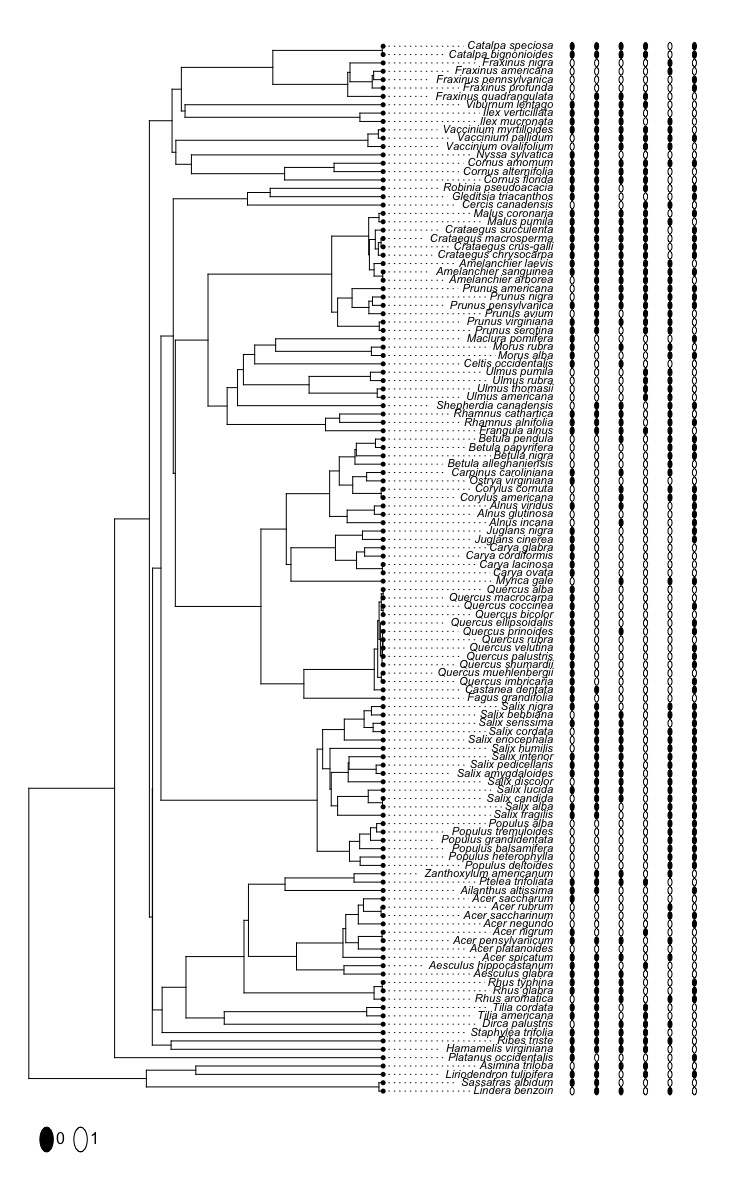
\includegraphics[width=12cm,height=12cm, keepaspectratio]{tree1.jpeg}} 
  \caption{This is my phylogeny, next to it all all the traits, I will have to explain these and label them}
  \label{Tree}
\end{figure}\\
\begin{figure}[H]
 \fbox{ 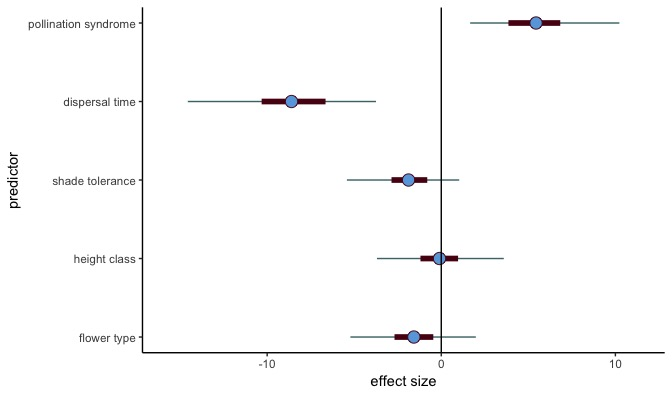
\includegraphics[width=\linewidth]{effect_plot2.jpeg}} 
  \caption{The effect size and significantce for each predictor, I'll explain this more too}
  \label{Effect sizes}
\end{figure}

\section{Suppliment}
full model with interactions
pp_checks?

\end{document}
